%----------------------------------------------------------------------------
\chapter{\bevezetes}
%----------------------------------------------------------------------------

Egy monitor feladata az, hogy futási időben egy rendszert megfigyeljen, elemezzen és egy adott követelmény alapján felismerje a rendszer helytelen viselkedését.
Ezt a helytelen viselkedést jelzi a rendszernek, de néhány esetben a rendszer működését is befolyásolhatja.
Egy rendszer viselkedése lehet kontextusfüggő, amit a monitornak figyelembe kell venni.
Például, egy gépjármű fékezésének vezérlését befolyásolja a terep, amin épp halad.
A rendszer működése tehát függ a környezetétől.
Ezért, hogy a viselkedését ellenőrizni tudjuk, a monitornak információval kell rendelkeznie a környezetben történő változásokról.
Ezen kívül, a monitornak időmérésre is szüksége van, mert a követelmény tartalmazhat időziteseket is.
Az 1.1. ábra bemutatja a monitorozás koncepcióját.

\begin{figure}[!ht]
    \centering
    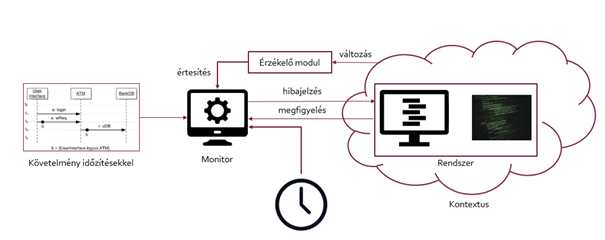
\includegraphics[width=150mm, keepaspectratio]{figures/1abra.png}
    \caption{Kontextusfüggő rendszerek monitorozása időzítési feltételekkel.}
\end{figure}

A scenario alapú monitorozás során a kommunikáció megfigyelésével szeretnénk felismerni a problémákat a rendszerünkben.
A rendszerben lévő objektumok közti interakciókat, üzeneteket fogja megfigyelni a monitor.
A követelményt scenario formájában adjuk meg az üzenet szekvenciák specifikálásához.
Szekvencia diagramok segítségével egyszerűen megadhatunk ilyeneket.
A diagramokat a későbbiekben olyan alakra kell majd hoznunk, hogy abból a monitor létrehozható legyen.

\begin{figure}[!ht]
    \centering
    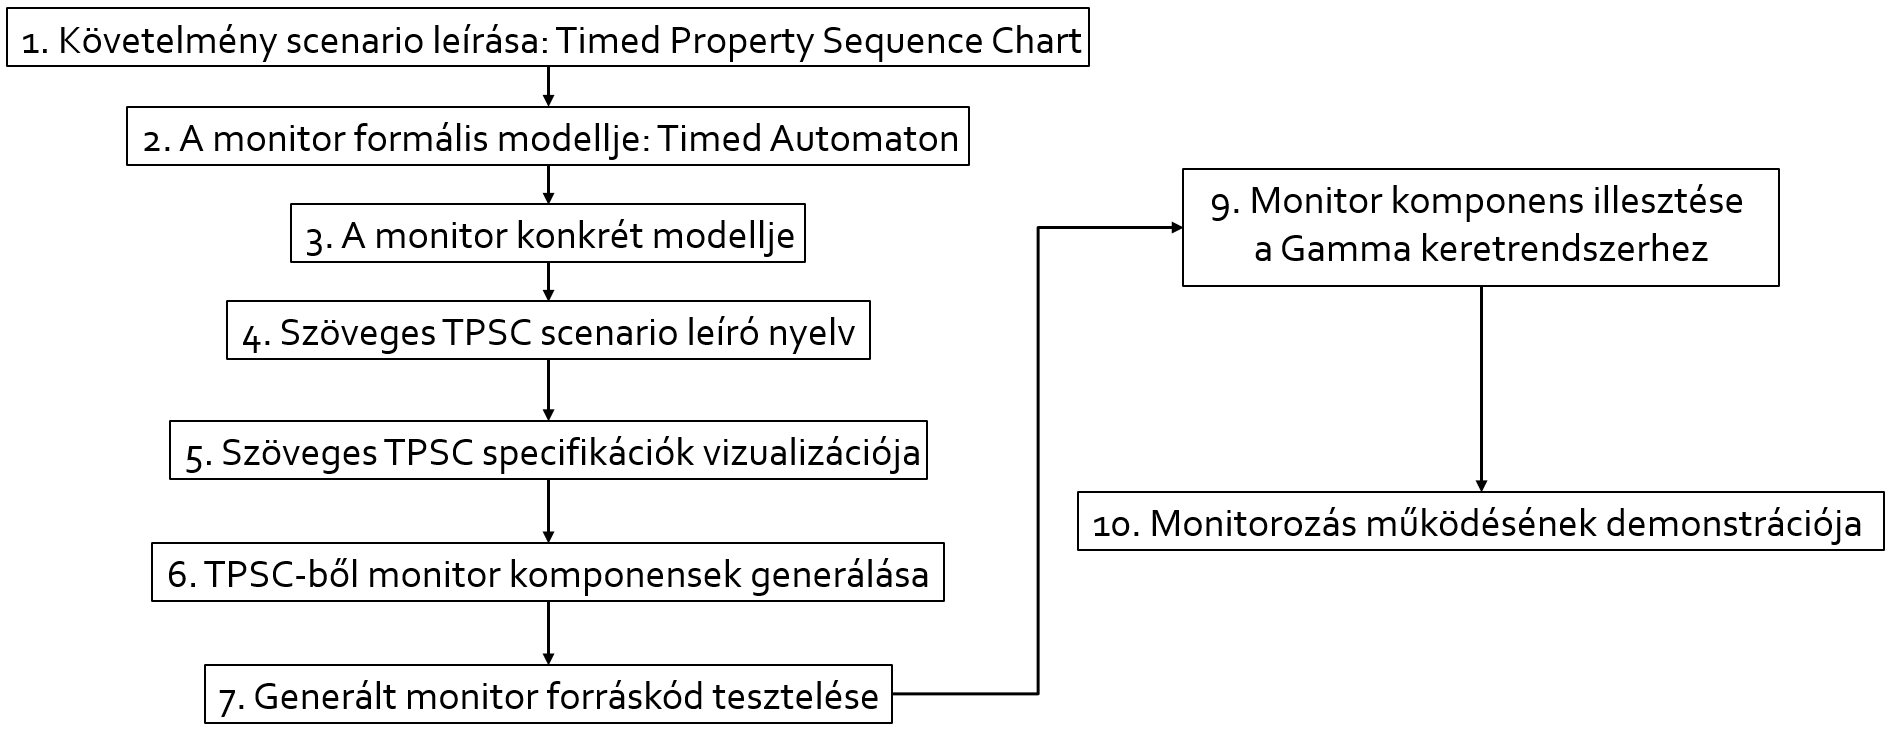
\includegraphics[width=150mm, keepaspectratio]{figures/generation_plan.png}
    \caption{Monitor generátor kibővítése.}
\end{figure}

A cél az, hogy a „Monitor komponensek generálása kontextusfüggő viselkedés ellenőrzése” című szakdolgozatom során elkészített monitor komponens generátort kibővíteni úgy, hogy támogassa időzítési feltételek megadását.
A monitor generálás terve látható a 5.1. ábrán.
Az Önálló laboratórium keretében az volt a feladatom, hogy a szakdolgozat során definiált szöveges PSC diagram leíró nyelvet kibővitsük a TPSC elemeivel.
Ezután az automata generátort kell úgy kibővíteni, hogy a TPSC diagramokból tudjon TA automatákat generálni.
Egy monitor forráskód generátor pedig az automata alapján elkészítheti a monitor forráskódját.

A szöveges TPSC scenario leírásához el kell készítenünk a diagram vizualizációját, hogy grafikusan megtekinthessük a definiál scenario-t.
A következő a generált monitor forráskód tesztelése, majd ezután ezt illeszük a Gamma keretrendszerhez.
Ezzel az a célunk, hogy elosztott komponens alapú rendszerek szimulációja közben monitorozható legyen a TPSC üzenet szekvencia specifikáció teljesülése illetve az ebben rögzített tulajdonságok megsértése

A Diplomatervezés 1 tárgy keretében a tervnek a negyedik, hatodik és hetedik részeivel foglalkoztam.
